\chapter{Modelling Returns}


\section{Returns as Random Variables}

We model stock returns as \textit{random variables}.
A random variable can take one of many values, with an 
associated probability. For example, the gross return on 
a stock can be one of four values as shown in Table \ref{tab:randomvariable}.

\begin{table}[!htbp]
    \centering
    \begin{tabular}{c c}
        % \hline
        $R$ & $\pi$ \\
        % \hline
        1.1 & 0.6 \\
        1.2 & 0.1 \\
        0.7 & 0.25 \\
        0.0 & 0.05 \\
    \end{tabular}
    \caption{Example of a gross return distribution.}
    \label{tab:randomvariable}
\end{table}

Each value is a possible \textit{realization}
of the random variable. You can experiment with this in Python
using the following code:

\begin{python}
import numpy as np

# Define the possible returns and their probabilities
returns = np.array([1.1, 1.2, 0.7, 0.0])
probabilities = np.array([0.6, 0.1, 0.25, 0.05])

# Generate a random return
print(np.random.choice(returns, size=1, p=probabilities))

\end{python}

Of course, stock returns can take on many more values 
than just four, but this is a simple example.

The \textit{distribution} of the random variable is 
a listing of the values it can take, along with their
associated probabilities. For example, the distribution
of the random variable in Table \ref{tab:randomvariable}
is:

\begin{figure}[!htbp]
    \centering
    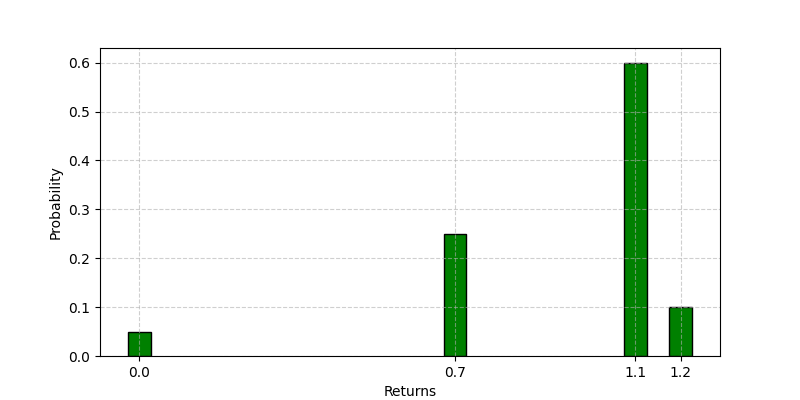
\includegraphics[width=0.8\textwidth]{randomvariables/fig1.png}
    \caption{Example of a random variable distribution.}
    \label{fig:randomvariable}
\end{figure}

Another way to think of a random variable is as a
\textit{function} that maps "states of the world" to
real numbers. For example, the random variable in 
Table \ref{tab:randomvariable} could be:

\begin{table}[!htbp]
    \centering
    \begin{tabular}{c c c}
        % \hline
        $R$ & States of the world & $\pi$ \\
        % \hline
        1.1 & New product works, competitor burns down & 0.6 \\
        1.2 & New product works, competitor ok. & 0.1 \\
        0.7 & Only old products work & 0.25 \\
        0.0 & Factory burns down, no insurance. & 0.05 \\
    \end{tabular}
    \caption{Random variable as a function mapping states of the world to real numbers.}
    \label{tab:statesoftheworld}
\end{table}

The probability really describes the external events 
that define the states of the world. Usually, we 
can't name those events, so we just use the probabilities
that the stock return takes on various values.

In the end, all random variables have a discrete number of values,
as in our example. Stock prices are only listed to 
1/8 dollar, all payments are rounded to the nearest cent, etc.
However, we often think of \textit{continuous} random variables,
that can be any real number. 
Corresponding to the discrete probabilities above,
we now have a continuous probability \textit{density},
usually denoted $f(R)$. 
The density tells you the probability per unit of $R$.
For example, $f(R_0)\Delta R$ tells you the probability
that the return is between $R_0$ and $R_0 + \Delta R$.

A common assumption is that returns (or log returns) are 
normally distributed. This means that the density is
given by the formula:

\begin{equation}
    f(R) = \frac{1}{\sqrt{2\pi\sigma^2}}\exp\left(-\frac{(R-\mu)^2}{2\sigma^2}\right)
\end{equation}

The graph of this function looks like this:

\begin{figure}[!htbp]
    \centering
    \begin{tikzpicture}
        \begin{axis}[
            axis lines=middle,
            xlabel={$R$},
            ylabel={$f(R)$},
            xtick=\empty, % Removes x ticks
            ytick=\empty, % Removes y ticks
            enlargelimits,
            clip=false,
            domain=-3:3,
            samples=100,
            ymin=0,
            ymax=0.45,
            % title={Normal Distribution of Returns}
        ]
        % Normal distribution parameters mu and sigma
        \def\mucomp{0}
        \def\sigmacomp{1}
        % Normal distribution formula
        \addplot[blue, thick] {1/(sqrt(2*pi*\sigmacomp^2)) * exp(-((x-\mucomp)^2)/(2*\sigmacomp^2))};
        
        % Adding mu label
        \node[pin={[pin edge={thick}, pin distance=0mm]90:{$\mu$}}] at (axis cs:\mucomp, 0) {};
    
        % Highlighting the spread influenced by sigma
        \draw[red, thick, <->] (axis cs:\mucomp-\sigmacomp,0.24) -- (axis cs:\mucomp+\sigmacomp,0.24)
            node[pos=0.5, fill=white] {$\sigma$};
    
    \end{axis}
    \end{tikzpicture}
    \caption{The probability density function of normally distributed returns}
\end{figure}

About $30\%$ ($31.73\%$ to be exact) of the probability 
of a normal distribution is more than one standard deviation
away from the mean. About $5\%$ of the probability is more
than two standard deviations away from the mean (in fact 
$4.55\%$, the $5\%$ probability lines is at 1.96 standard deviation).
That means that there is only one chance in 20 that the return
will be more than two standard deviations away from the mean 
in a normally distributed world. In reality, stock returns 
have "fat tails", meaning that they are more likely to take 
on extreme values than a normal distribution would suggest.

You can experiment modelling returns with
a normal distribution in Python:

\begin{python}
import numpy as np

# Parameters for the normal distribution
mu = 1  # Mean
sigma = 0.05  # Standard deviation

print(np.random.normal(mu, sigma, 1))
\end{python}

\section{Expected Value and Variance of Returns}

Rather than plot the entire distribution, 
we usually summarize the behavior of a random variable
with two numbers: the \textit{mean} and the
\textit{variance}.

We denote the values that $R$ can takes on a $R_i$, 
with associated probabilities $\pi_i$. 
The mean of $R$ is given by:

\begin{equation}
    E(R) = \sum_i R_i \pi_i
\end{equation}

The mean is a measure of \textit{central tendency}.
It tells you where $R$ is on average. A high mean
stock return is obviously better than a low mean
stock return.

The \textit{variance} of $R$ is given by:

\begin{equation}
    \sigma^2(R) = E[(R - E(R))^2]
    = \sum_i \pi_i(R_i - E(R))^2
\end{equation}

Since squares are always positive, variance tells 
you how much $R$ is far away from its mean. It 
measures the spread of the distribution. High 
variance is not a good thing. It will be 
our measure of \textit{risk}.